\documentclass[11pt,a4paper,oneside]{article}
\usepackage[latin1]{inputenc}
\usepackage{amsmath}
\usepackage{amsfonts}
\usepackage{amssymb}
\usepackage{graphicx}
\usepackage{color}
\usepackage {tikz}
\usetikzlibrary {er}
\usepackage[left=2.00cm, right=2.00cm, top=1.00cm]{geometry}
\graphicspath{{./}}

\begin{document}
	\title{DS 221 - Introduction to Scalable Systems \\ Assignment 2}
	\author{Shriram R. \\ M Tech (CDS) \\ 06-02-01-10-51-18-1-15763}
	\maketitle
	
	\section{Searching}
	The dictionary abstract data structure has been implemented by hash map, unsorted arrray and sorted array. Time complexities for Insert and Lookup performance has been analyzed and empirically verified. The following sections will cover the analysis and empirical results in detail.
	
	\subsection{Hash Table}
	Let C denote the capacity or number of buckets in the hash table and N denote the total number of records in the hash table. Collisions are resolved by chaining of key-value records. K mod C is the hash function used where K is the key value.\\
	\newline
	In the case of insertion, a new record would be added to the end of the chain (STL list) of its bucket. The time complexity for this insertion is O(1). Hence, insertion of N records take O(N) time. This is independent of the key distribution. \\
	\newline
	For uniform distribution of keys, each bucket would have $\frac{N}{C}$ records on average. Hence, the time complexity to search a record is $O(\frac{N}{C})$. For non-uniform ditribution, the worst case time complexity is O(N). This happens when all the records are present in a single bucket. However, if the maximum number of records in a bucket is bounded by M ($<$N), then the worst case time complexity id O(M).
	
	\begin{center}
		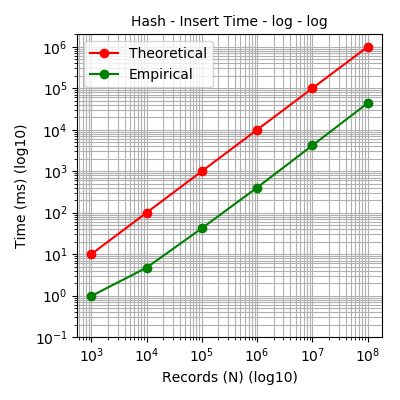
\includegraphics[scale=0.6]{1.png}		
	\end{center}

    \begin{center}
    	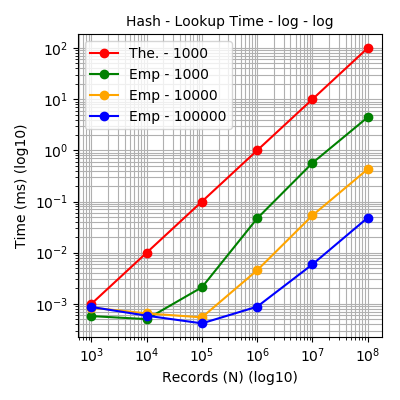
\includegraphics[scale=0.6]{2.png}		
    \end{center}
	
	It is observed that the insert time is consistent with theoretical analysis. The lookup time is consistent for large values of N but deviates from the analytical model for lower N values. This is could be due to caching and locality which is not captured in the theoretical model.
	
	\subsection{Unsorted Array}
	Insertion for each record can be done in O(1) time since a new record is added to the end of the array. Hence, the time complexity to insert N records would be O(N). \\
	\newline
	For lookup, linear scan is performed over the entire array till the last record since the records are not sorted by key. Hence, the worst case time complexity for lookup is O(N). Note that the insert and lookup time is independent of key distribution.
	
	\begin{center}
		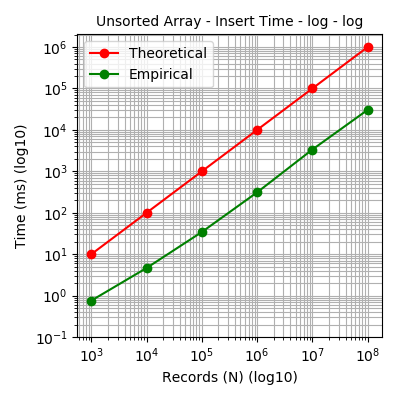
\includegraphics[scale=0.6]{3.png}		
	\end{center}
	
	\begin{center}
		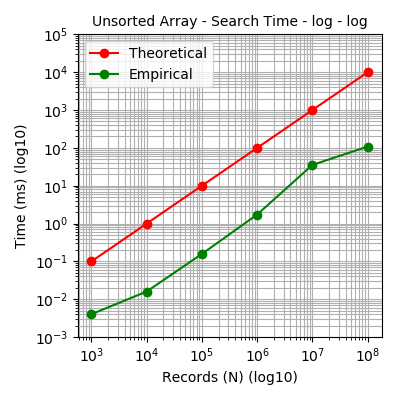
\includegraphics[scale=0.6]{4.png}		
	\end{center}

    From the emprical results, it can be observed that the time taken generally agrees with the analysis. There is a minor deviation of lookup time from the theoretical value which could be due to cache effects and inaccuracies in measuring the lookup time.
	
	\subsection{Sorted Array}
	Insertion of records takes O(N) time similar to that of unsorted array but there is an additional step at the end of insertion which sorts the records by key. This takes an additional O(N log N) time. So, the total time is O(N log N). \\
	\newline
	For lookup, binary search of the lookup key is performed on the sorted array. The time complexity for this binary search is O(log N). Similar to sorted array, the lookup and insert time is independent of key distribution. 
	
	\begin{center}
		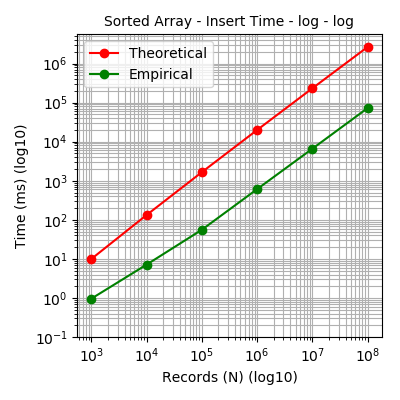
\includegraphics[scale=0.6]{5.png}		
	\end{center}
	
	\begin{center}
		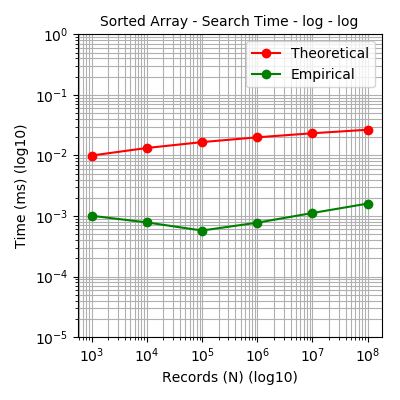
\includegraphics[scale=0.6]{6.png}		
	\end{center}
     
     It is observed that the insert time is consistent with theoretical analysis. The lookup time marginally deviates from the theoretical value for lower N values. This could be due to caching and inaccuracies in capturing the time for lookup.  
     
    \subsection{Comparison}
    The table given below show the theoretical complexities of the above implementations. It can be inferred that Unsorted array is the worst choice in terms of lookup time. Hash table is better than sorted array in terms of lookup if the bucket count C is greater than $\frac{N}{log N}$. Hash table is also faster for inserts than sorted array.
     \begin{center}
     	\begin{tabular}{|c|c|c|}
     		\hline 
     		\textbf{Implementation} & \textbf{Insert} & \textbf{Lookup} \\
     		\hline
     		Hash Table & O(N) & O($\frac{N}{C}$) \\ 
     		\hline 
     		Unsorted Array & O(N) & O(N)\\ 
     		\hline 
     		Sorted Array & O(N log N) & O(log N)\\ 
     		\hline 
     	\end{tabular}
     \end{center}
     
    
    \subsection{Note on Empirical Analysis}
    The empirical testing was done on a compute node in the Turing cluster having 8 core processor clocked at 2.6 GHz and 32GB RAM. Test data was generated using custom scripts available at [4].
    
    \subsection{Note on Code}
    The IDictionary.h file contains the definition of the given interface. The DictImpl.cpp file contains three different implementation of the given interface.  The Runner.cpp contains the driver code for the implementation. The Makefile can be used to generate the Runner.o file.
    
    \subsection{References}
    
\end{document}